\documentclass[10pt,twocolumn,letterpaper]{article}

\usepackage{cvpr}
\usepackage{times}
\usepackage{epsfig}
\usepackage{graphicx}
\usepackage{amsmath}
\usepackage{amssymb}
\usepackage{graphics}
\usepackage{subfigure}
\usepackage{amssymb}
\usepackage{amsthm}
\usepackage{amsmath}
\usepackage{algorithm}
\usepackage{algorithmic}
\DeclareMathOperator*{\argmin}{argmin}
% Include other packages here, before hyperref.

% If you comment hyperref and then uncomment it, you should delete
% egpaper.aux before re-running latex.  (Or just hit 'q' on the first latex
% run, let it finish, and you should be clear).
\usepackage[breaklinks=true,bookmarks=false]{hyperref}

\cvprfinalcopy % *** Uncomment this line for the final submission

\def\cvprPaperID{****} % *** Enter the CVPR Paper ID here
\def\httilde{\mbox{\tt\raisebox{-.5ex}{\symbol{126}}}}

% Pages are numbered in submission mode, and unnumbered in camera-ready
%\ifcvprfinal\pagestyle{empty}\fi
\setcounter{page}{1}
\begin{document}

%%%%%%%%% TITLE
\title{Fully Convolutional Attention Localization Network: Efficient Fine-Grained Recognition by Zooming in on Attention Regions}

\author{Xiao Liu, Tian Xia, Jiang Wang and Yuanqing Lin\\
Baidu Research\\
{\tt\small \{liuxiao12,xiatian,wangjiang03,linyuanqing\}@baidu.com}
}

\maketitle
%\thispagestyle{empty}

%%%%%%%%% ABSTRACT
\begin{abstract}
Fine-grained recognition is challenging mainly because the inter-class differences are usually local and subtle.
In order to distinguish them from the intra-class variations, it is essential to zoom in on highly discriminative local regions.
In this work, we introduce a reinforcement learning-based fully convolutional attention localization network to adaptively select multiple task-driven visual attention regions.
We show that zooming in on the selected attention regions significantly improves the performance of fine-grained recognition.
Compared to previous reinforcement learning-based models \cite{bd1,bd2,bd3}, the proposed approach is significantly faster during both training and testing because of its fully-convolutional architecture, and it can simultaneous focus its glimpse on multiple visual attention regions.
The experiments demonstrate that the proposed method achieves notably higher categorization accuracy on three benchmark fine-grained recognition datasets: Stanford Dogs \cite{bd4}, Stanford Cars \cite{bd5}, and CUB-200-2011 \cite{bd6}.
\end{abstract}

%%%%%%%%% BODY TEXT
\section{Introduction}
Fine-grained recognition refers to the tasks of distinguishing sub-ordinate categories, such as bird species, dog breeds, and car models. It is an important topic to make computer rivals human experts in visual understanding.
Compared to generic object recognition, fine-grained recognition is more challenging.
The discriminative features to recognize fine-grained classes are typically not just on the whole object but also on multiple object parts.
Therefore, it requires us to both locate the parts that contain discriminative details and differentiate fine details in appearance.

Most conventional methods~\cite{bd10,bd15} utilize manually defined parts to localize the regions for fine-grained recognition, such as ``the head of a bird''.
However, relying on manually defined parts has several drawbacks: 1) the precise part annotations is time-consuming and expensive.
2) The strongly supervised part-based model might fail if  some parts are occluded in the image.
3) Finally but most importantly, there is no clue that manually defined parts are optimal for any fine-grained recognition task.
For example, it is very difficult to define parts to recognize food.


Instead, visual attention approaches~\cite{bd3} utilizes reinforcement learning-based visual attention model~\cite{bd1} to simultaneous learn to localize object parts and classify object within scene.
The model learns a task-driven policy to localize the object parts via a set of {\em glimpse}.
Each glimpse takes a multi-resolution crop of the image, and outputs the next glimpse location and possibly the next object part.
The whole framework can be learned in an end-to-end way by REINFORCE algorithm~\cite{bd20}, where the location of each glimpse is an action.
This approach requires no manual part annotations, and are trained end-to-end by reinforcement learning (RL).
This framework simulate the recognition process of human vision system.
Moreover, the visual attention approach is demonstrated to perform well on fine-grained recognition without requiring manually labeled object parts~\cite{bd3}.
However, it is computationally expensive during both training and testing, because it  needs to individually run a neural networks on each image crop.


In this paper, we propose a novel framework called Fully Convolutional Attention Localization Network.
It is a computationally efficient reinforcement learning-based framework to learn task-driven policies for attention localization.
In this framework, multiple glimpses are produced by passing the image to a fully convolutional neural network~\cite{bd7, bd8}.
The fully convolutional neural network generates multiple score maps given the image and the score maps of the last glimpses.
Each score map corresponds to an object part and can have different resolutions.
The location with the maximum score is utilized as the attention region of the corresponding part for the next glimpse.


The attention localization network enjoys very fast training and testing, because of its fully-convolutional architecture and feature sharing techniques.
The convolutional neural network is shared across multiple glimpses, and the convolutional neural networks of all the parts are also shared in a way similar to Fast-RCNN~\cite{girshick2015fast}.
It also converges faster than previous RL-based methods~\cite{bd1,bd2,bd3} on large datasets.
The proposed approach also significantly outperforms state-of-the-art reinforcement learning-based approaches in fine-grained recognition because it can simulataneously locate multiple parts.

We perform experimental evaluation on three publicly available datasets: Stanford Dogs \cite{bd4}, Stanford Cars \cite{bd5} and CUB-200-2011 \cite{bd6}.
The experiments demonstrate that we can improve the performance significantly over state-of-the-art reinforcement learning based methods without utilizing complicated model fusion techniques.
It also outperforms most previous strongly supervised methods on Stanford Dogs ($84.1\%$).

The remainder of the paper is organized as follows. The related work is reviewed in Section 2.
The fully convolutional attention localization network is described in Section 3.
The process of model training is described in Section 4.
Performance studies and experimental analysis are illustrated in Section 5.
The conclusion and future work is presented in Section 6.

\section{Related Work}
\subsection{Fine-Grained Recognition}
Fine-grained recognition algorithm relies on part localization~\cite{bd9,bd10,bd11,bd12,bd13,bd14} to focus on the important regions and discriminative representation learning to distinguish the subtle difference.

Part localization-based fine-grained recognition algorithms localize object parts, which can either be manually defined or automatically found using data mining techniques.
Most of the algorithms employs manually defined object parts.
Berg et al. \cite{bd9} learn a set of intermediate features using data mining techniques.
Each feature discriminates two classes based on the appearance of a particular part.
Liu et al. \cite{bd10} employ the local appearance features of manually defined parts, such as face and eyes, and combine them with global features for dog breed classification.
The experimental results show that accurate part localization significantly increases classification performance.
Zhang et al. \cite{bd11} utilize part-based R-CNNs as whole-object and part detectors to detect the pose of the objects.  The CNN appearance representation is then pose-normalized for fine-grained recognition.

There have also been a few works that find discriminative parts in an unsupervised way.
Yang et al. \cite{bd12} propose a template model that discovers the common geometric pattern of object parts and the co-occurrence statistics of the patterns.
Features are extracted within the aligned co-occurred patterns for fine-grained recognition.
Similarly, Gavves et al. \cite{bd13} and Chai et al. \cite{bd14} segment images and align the image segments in an unsupervised fashion, then they extract features for each aligned image segment.

Successful fine-grained recognition also calls for discriminative representation learning to learn appearance feature.
Most of the current state-of-the-art fine-grained recognition algorithms are based on deep CNN representation.
Branson et al. \cite{bd15} claims that integrating lower-level layer features and higher-level layer features learns more discriminative representation for fine-grained recognition.
Lin et al. \cite{bd16} propose a bilinear architecture to model local pairwise feature interactions for fine-grained recognition, where convolutional features from two models are combined in a translation invariant manner.
Qian et al. \cite{bd17} propose a multi-stage metric learning framework to learns a distance metric that pulls data points of the same class close and pushes data points from different classes far apart.
Wang et al. \cite{bd18} combine saliency-aware object detection approach and object-centric sampling scheme to extract more robust and discriminative features for large-scale fine-grained car classification.

Although these works have achieved significant progress on fine-grained recognition and demonstrated the importance of part localization and discriminative representation learning, they generally treat these two parts separately.

\subsection{Attention Model}
Several works introduce attention-based models for task-driven object/part localization.
Mnih et al. \cite{bd1} present a recurrent neural network model for object detection by adaptively selecting a sequence of attention regions and extract appearance  representations in the these regions.
Since this model is non-differentiable, it  is trained with reinforcement learning techniques to learn  task-specific policies.
Ba et al. \cite{bd2} extend Mnih et al.'s work and successfully achieve good results on a more challenging multi-digit recognition task.
Sermanet et al.~\cite{bd3} further extend \cite{bd2} and present experiments on fine-grained recognition datasets.
Jaderberg et al.~\cite{jaderberg2015spatial} proposes an differentiable attention mechanism that can be trained without reinforcement learning.

Compared to previous approaches, the recurrent attention models \cite{bd1,bd2,bd3} have remarkable contributions to fine-grained recognition problem,
because they can learn the part localization and discriminative representation in an end-to-end way, and they do not require manually labeled object parts.
However, they also suffer from several drawbacks in practice. First, they only result in small performance improvement.
\cite{bd3}  achieves 76.8\% mean accuracy percentage (with 3 glimpses) on Stanford Dogs dataset while the result of GoogLeNet \cite{bd7} baseline is 75.5\%.
Second, the computational burden is high.
\cite{bd3} employs GoogLeNet for representation learning. However, calculating the features at each glimpse requires forwarding GoogLeNet three times, leading to very slow training and testing.

In contrast, the proposed framework has several advantages.
\begin{itemize}
\item {\bf Computational Efficiency:} It is much more computationally efficient because of the fully convolutional neural network architecture and feature sharing techniques.
\item {\bf Multiple Part Localization:} It is capable of localizing multiple parts with different sizes simultaneously for fine-grained recognition.
\end{itemize}

As a result, the proposed framework not only achieves significant improvements over state-of-the-art methods on several benchmark datasets,
it is also more suitable to be applied to practical applications where the dataset is usually much larger because of its computational efficiency.

% \begin{itemize}
% \item \textbf{Small performance improvement.} \cite{bd3}  achieves 76.8\% mean accuracy percentage (with 3 glimpses) on Stanford Dogs dataset while the result of GoogLeNet \cite{bd7} baseline is 75.5\%. Considering the attention-based model is much more complicated, the improvement is slight.

% \item \textbf{High computational burden.} \cite{bd3} employs GoogLeNet for representation learning. However, calculating the features at each glimpse requires forwarding GoogLeNet three times, leading to very slow training and testing.

% %\item \textbf{Convergence difficulty.} Because the attention-based models\cite{bd1,bd2,bd3} are trained with reinforcement learning, the convergence of the model is slow and heavily depends on the exploration parameters.
% \end{itemize}

% In contrast to the above works, the training and testing of the proposed work is much faster, and the recognition accuracy significantly outperforms the baseline methods.

\section{Attention Localization Network}

\begin{figure*}[!t]
\begin{center}
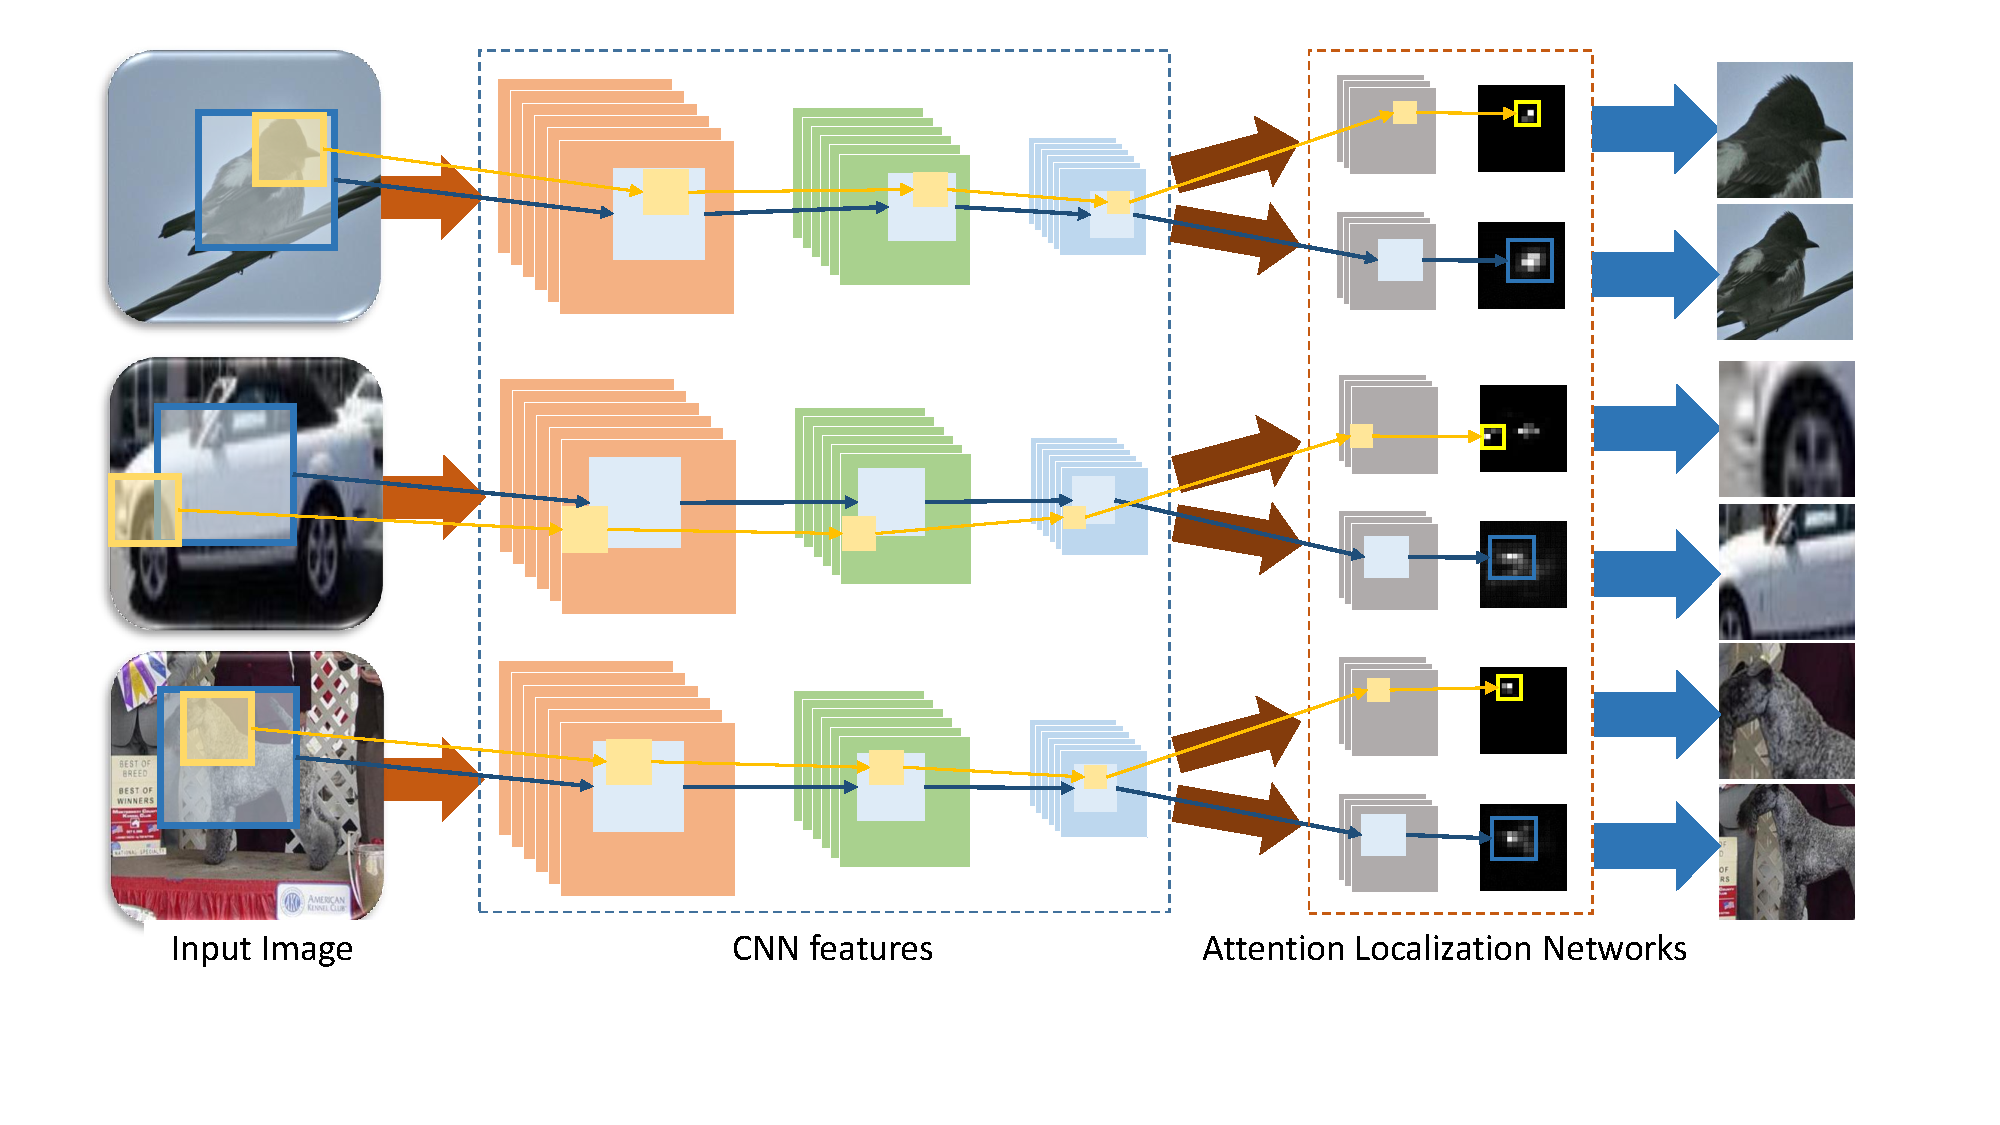
\includegraphics[scale = 0.55]{1.pdf}
\end{center}
\caption{The architecture of the attention localization network. In this example, the attention localization network finds two parts with different sizes (the blue region and the yellow region).
Both parts are localized using the same convolutional feature map.
}\label{fig:architecture}
\end{figure*}

Fig.~\ref{fig:architecture} illustrates the architecture of the attention localization network.
The attention localization network can localize multiple object parts using attention mechanism.
Different parts can have different sizes that are manually defined.

Given an input image, we extract basis convolutional feature maps using the VGG 16 model \cite{bd8} pretrained on ImageNet dataset~\cite{bd19} and fine-tuning for the target fine-grained dataset.
The attention localization network localizes multiple parts by generating a score map for each part using  the basis convolutional feature map.
Each score map is generated using two stacked convolutional layers and one spatial softmax layers.
The first convolutional layer uses 64 $3\times3$ kernels, and the second one uses one $3\times3$ kernels to output a single-channel confidence map.
This confidence map is combined with all the confidence maps of the last time step to generate the final confidence map.
The spatial softmax layer is applied to the final confidence map to convert the confidence score into probability.
The attention region with highest probability is selected as the part location.

A local image region is cropped around each part location.
The size of image regions cropped for different parts might be different.
We train an image classifier for each local image region as well as the whole image individually.
The final classification results is the average of all the classification results from the individual classifiers.

In order to discriminates images based on small differences, the local image regions is resized to its high resolution.
A separate deep convolutional neural network is trained for each part for classification.


Although resizing the local image regions can achieve good classification performance, it requires us to perform multiple forward and backward passes of $N$ very deep convolutional neural network in one training batch,
where $N$ is the number of parts.
This is too time-consuming in practice.
Thus, we employ an approximated part classification method that is similar to Fast-RCNN~\cite{girshick2015fast}.
In order to improve the training speed, one important characteristic of the proposed architecture is that the convolutional feature maps for part localization, part classification, and whole image classification are shared during training.
The convolutional features for each part is obtained by selecting the corresponding region in the convolutional feature map of the whole image, so that the receptive field of the selected region is the same as the size of the part.
The convolutional features for each time steps are also shared.
As a result, we only need to run the forward pass of the deep convolutional once in one training batch.
Notice that these classification networks are only utilized to obtain the reward during attention localization network training.
The final classification networks are based on the resized high resolution images.

\subsection{Inference}
We now describe how to utilize the attention localization network for fine-grained recognition during inference.
Given an image, we first localize multiple attention regions by selecting the location with highest probability for each part in attention localization network in the last timestep.
We then focus on each part's location by resizing the regions around it to its corresponding high resolution.
Each resized part region as well as the original image makes the prediction individually.
The final prediction score is the average of the prediction scores from the original image and all attention regions.


\section{Training Attention Localization Networks}
Since there are no ground-truth annotations to indicate where to select attention regions, we adopt reinforcement learning to learn the parameters of the attention localization networks.

In particular, the entire attention localization problem is formulated into Partially Observable Markov Decision Processes (POMDPs).
During each step of POMDP, an attention localization network works as an agent to perform an action based on the observation and receives a reward.
In our work, the action corresponds to the location of the attention region, the observation is the input image, and the reward measures the quality of the classification using the attention region.
The target of our learning is to learn the optimal decision policies, characterized by the parameters of the attention localization networks, to maximize the sum of expected reward of all the time-steps.

Since the rewards cannot be directly obtained in our work, additional auxiliary classification networks are trained to measure the classification quality.

The classification network in each step is a fully-connected layer followed by a softmax layer, which uses the convolutional features of all previous selected attention regions as the input.
It should be noted although the convolutional feature maps are shared, the feature dimensions of attention regions in different steps are distinct because their sizes are different.

The classification networks and the attention localization networks are jointly optimized to maximize the following objective function:
\begin{equation}
J(\theta_L, \theta_C) =  R(\theta_L) - \lambda L(\theta_C),
\end{equation}
where $\theta_L, \theta_C$ are the parameters of attention localization networks and classification networks, respectively.  $\lambda$ is a balance weight,  $L(\theta_C)$ is the cross-entropy classification loss, and
\begin{equation}
R(\theta_L) = \frac{1}{NT}\sum_{n=1}^{N}\sum_{t=1}^T E_{\theta_L}(r_{n,t})
\end{equation}
is the average expected reward over $N$ training samples and $T$ different selection regions.

\begin{equation}
E_{\theta_L}(r_{n,t}) = \int_{A_{n,t}} p_{\theta_{L,t}}(A_{n,t}|x_n)r(A_{n,t})
\end{equation}
is the expected reward of the t-th selected attention region of the n-th sample,
where $\theta_{L,t}$ is the parameters of the t-th attention localization network,
$x_n$ is the n-th input image, and $A_{n,t}$ is the t-th selected region.
$p_{\theta_{L,t}}(A_{n,t}|x_n)$, the probability to selecting $A_{n,t}$ as attention region given by the attention network.
The reward $r(A_{n,t})$ is crucial for developing an efficient learning algorithm. We will describe the design of the reward in the following subsection.

\subsection{Reward Strategy}
A straightforward reward strategy is to measure the policy quality of selected attention regions of an image as a whole, i.e., $r(A_{n,t}) = 1$  if $t = T$ and the image is correctly classified, and 0 otherwise. Although the POMDP with such strategy can be learned in a recurrent way \cite{bd1}, it confuses the effects of selected regions in different steps, and involves in the problem of convergence difficulty.

We consider an alternative reward strategy, namely greedy reward, to handle the convergence problem
\begin{equation}
r(A_{n,t})=\left\{\begin{array}{ccc} 1 & : & t = 1 \wedge c_{n,1} = y_{n} \\ 1 &:& t > 1 \wedge c_{n,t} = y_{n} \wedge l_{n,t} < l_{n,t-1} \\ 0&:& otherwise   \end{array}\right.
\end{equation}
where $c_{n,t}$ is the predicted classification result, $y_{n}$ is the ground-truth label, and $l_{n,t}$ is the classification loss. If the image is classified correctly in the first step, the attention localization network immediately receives a reward. In other steps, we reward the corresponding attention localization network only if the image is classified correctly and the classification loss decreases with regards to the last timestep.
Otherwise, the attention localization network receives zero reward.

Compared to \cite{bd1} that maximizes the expected sum reward of a $T$-step POMDP, our approach can be seen as maximizing the expected sum reward of $T$ individual POMDPs, such that the possible parameter space is much smaller and the model is easier to converge.

\subsection{Optimization}

\begin{figure}[htb]
  \begin{center}
    \subfigure[Forwarding]{
    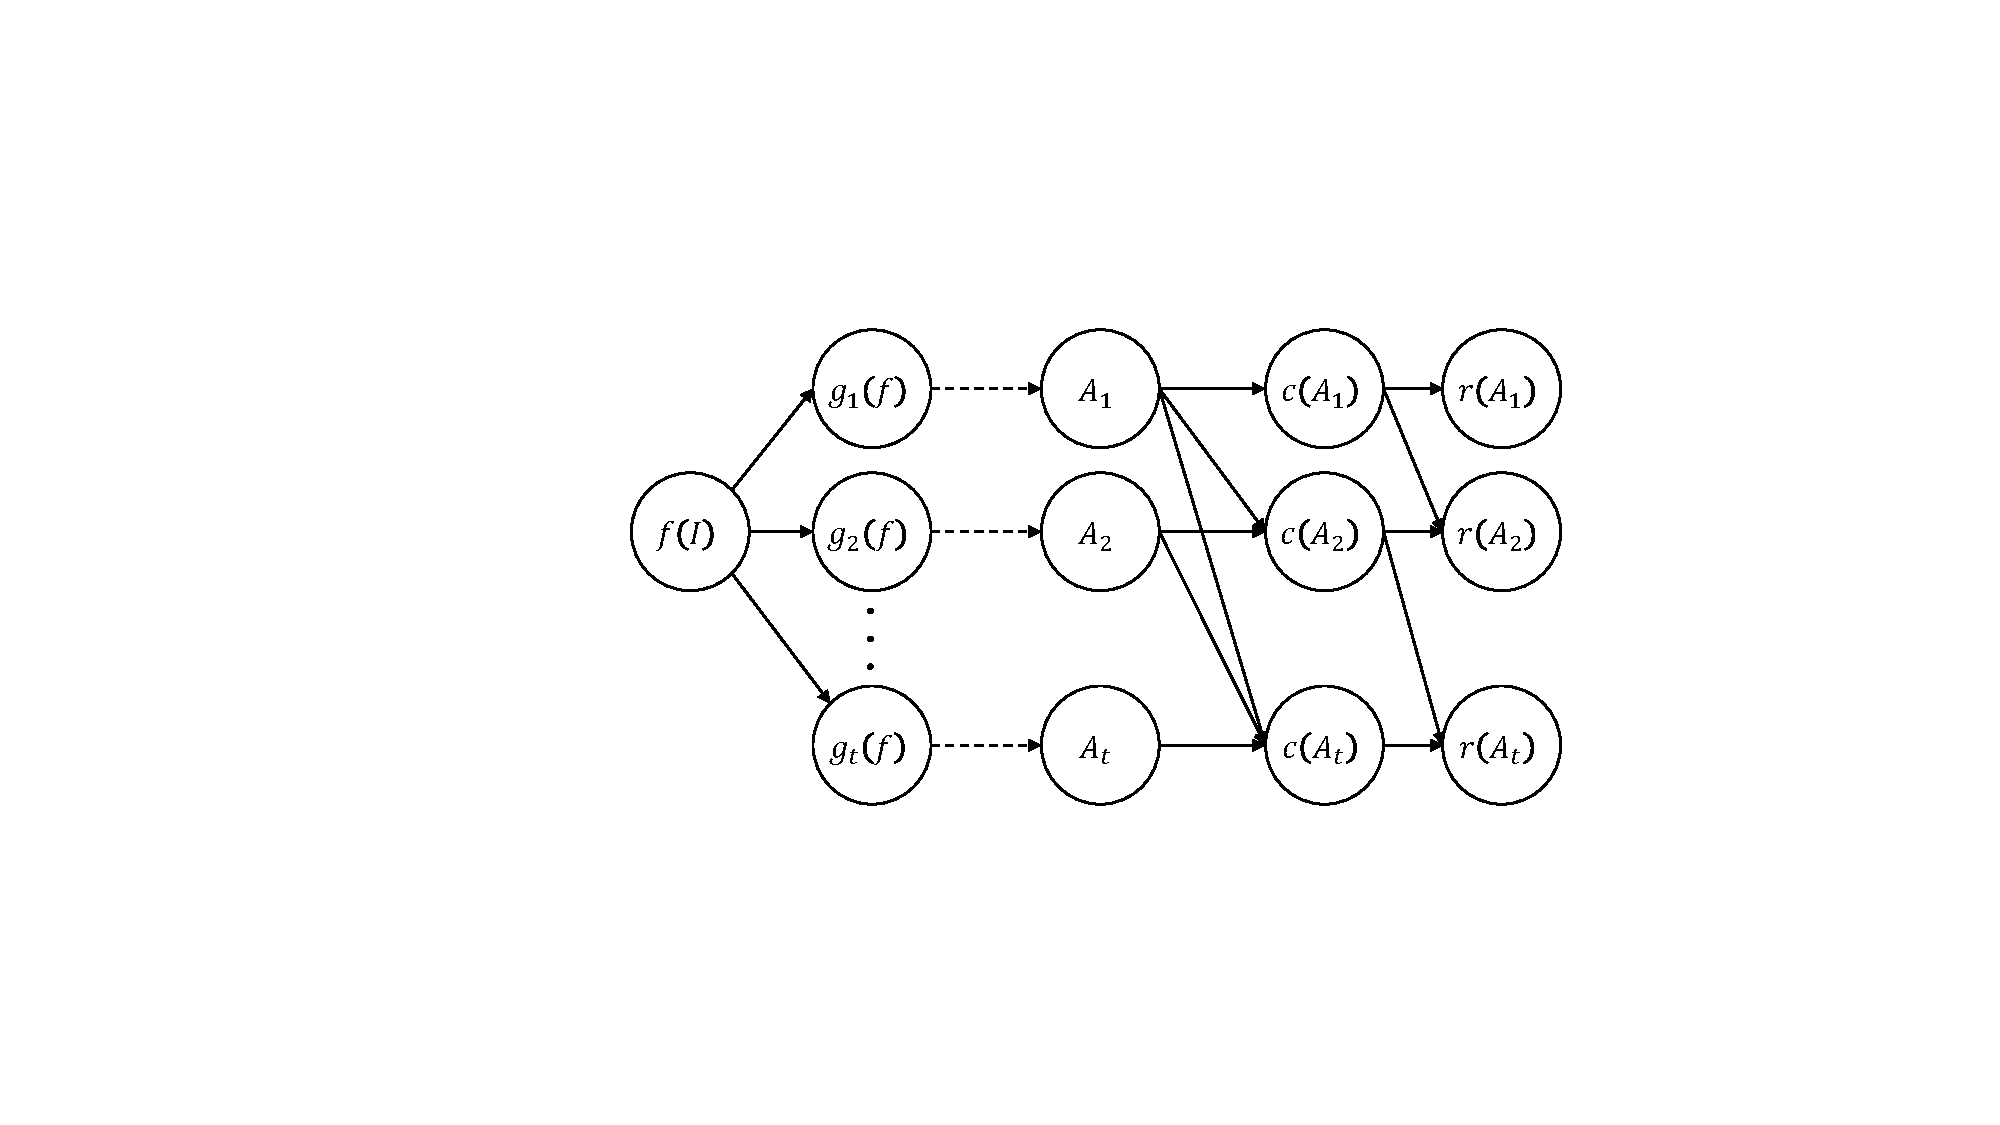
\includegraphics[scale = 0.4]{2-1.pdf}}
    \hspace{0.05in}%
    \subfigure[Back-propagation]{
    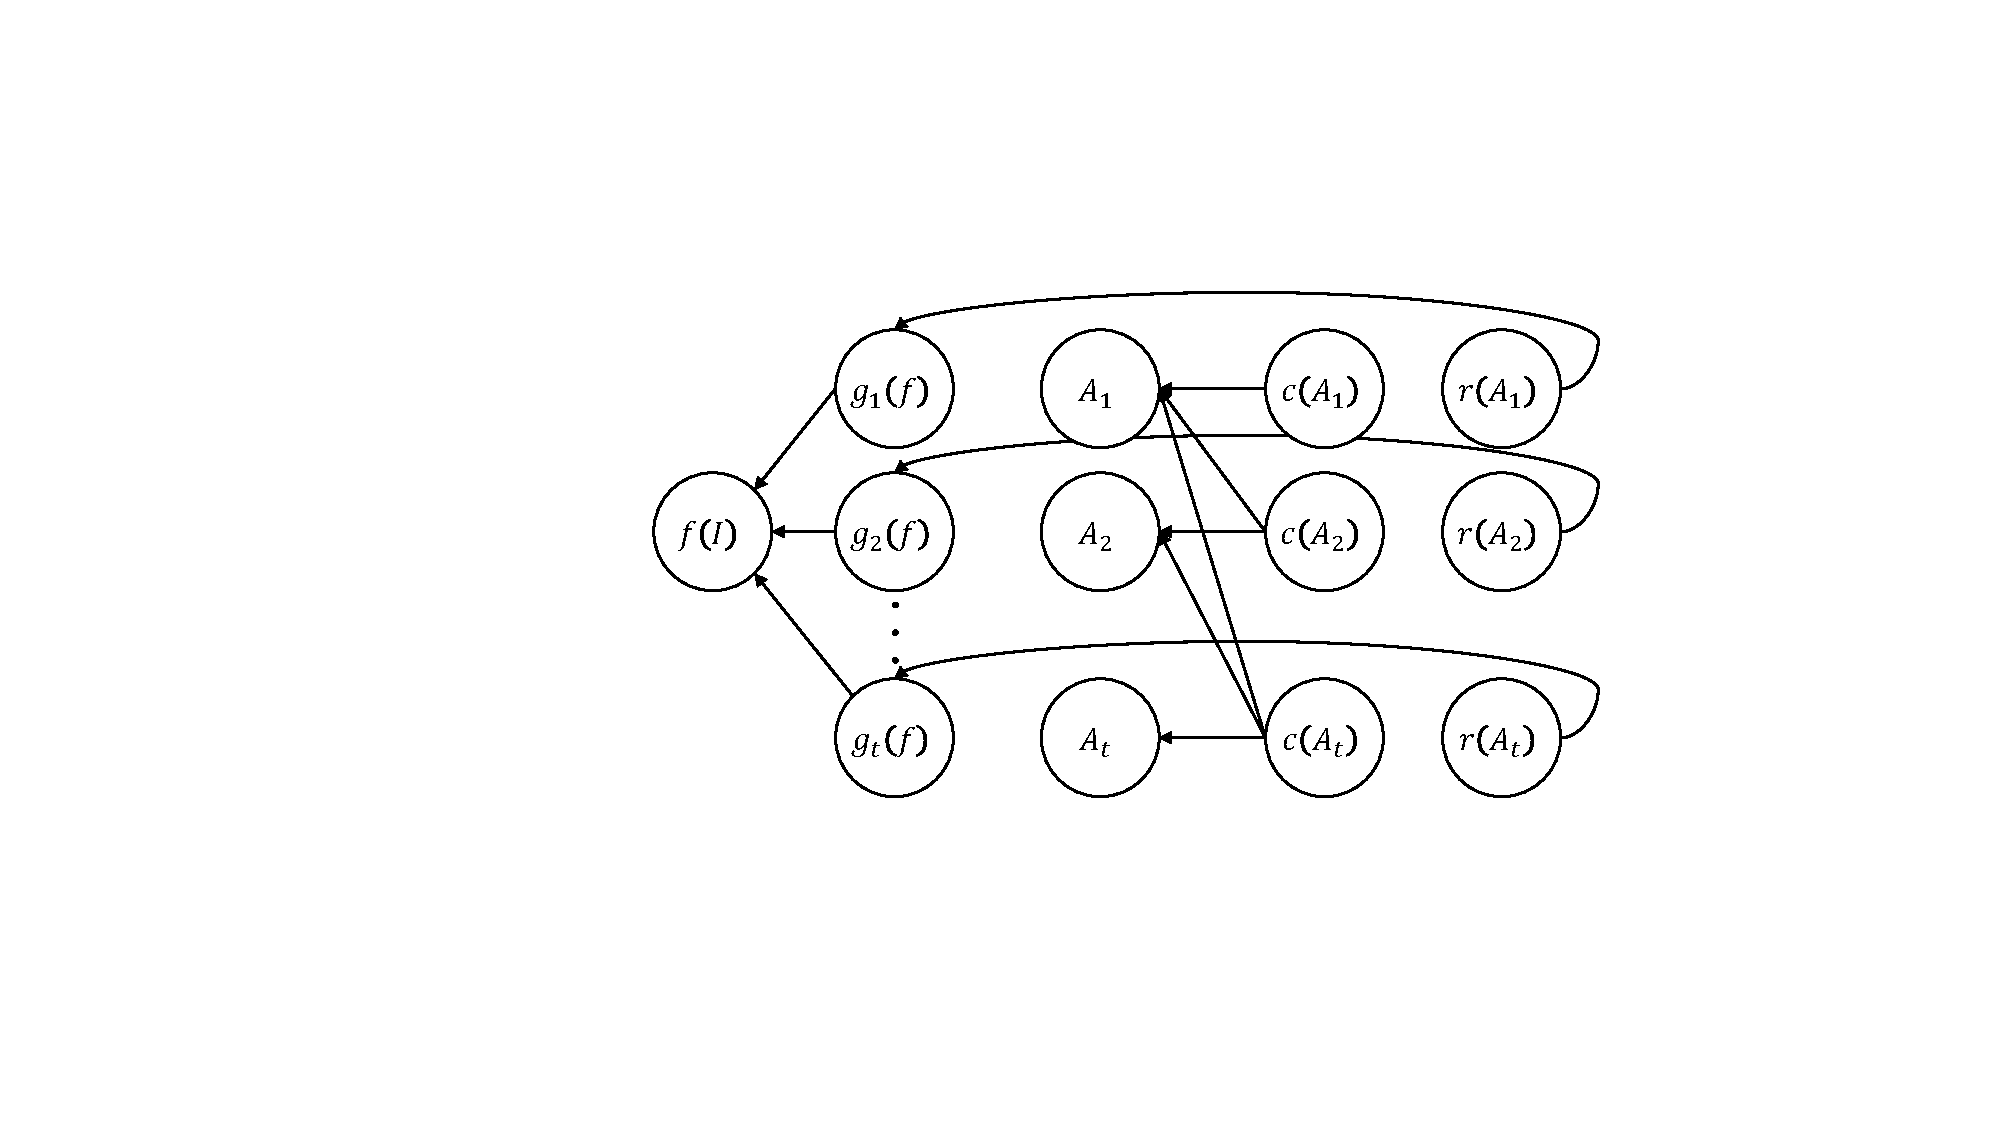
\includegraphics[scale = 0.4]{2-2.pdf}}
  \end{center}
\caption{The forwarding (a) and back-propagation (b) processes for training attention localization networks as POMDPs. The dashed lines indicate the sampling procedures. }
\end{figure}

It is difficult to directly calculate the gradient of $E_{\theta_L}(r_{n,t})$ over $\theta_L$ because it requires evaluating exponentially many possible part locations during training.
As shown by \cite{bd20}, the gradient can be approximated in a Monte Carlo way:
\begin{eqnarray}
\partial (p_{\theta_{L,t}}(A_{n,t}|x_n)r(A_{n,t})) \hspace{1.3in}\\
= p_{\theta_{L,t}}(A_{n,t}|x_n) \partial (\log p_{\theta_{L,t}}(A_{n,t}|x_n)r(A_{n,t})) , \nonumber
\end{eqnarray}
Thus,
\begin{eqnarray}
\partial E_{\theta_L}(r_{n,t}) \hspace{2.1in}\\
 = \int_{A_{n,t}} p_{\theta_{L,t}}(A_{n,t}|x_n) \partial (\log p_{\theta_{L,t}}(A_{n,t}|x_n)r(A_{n,t})) \hspace{-0.215in} \nonumber\\
 \approx \frac{1}{K} \sum_{k=1}^K \partial(\log p_{\theta_{L,t}}(A_{n,t}^k|x_n)r(A_{n,t}^k)) \hspace{0.5in} \nonumber
\end{eqnarray}
where $A_{n,t}^k\sim p_{\theta_{L,t}}(A_{n,t}|x_n) $ is sampled according to a multinomial distribution parameterized by the output confidence map of the attention localization network.

The forwarding process of training the attention localization networks as POMDPs is shown in Figure 2(a). Given basis conv features $f(I)$ as input, the attention networks output the confidence map $g_t(f)$ for different time step. Each confidence map $g_t(f)$ forms a multinomial distribution, and the location of attention region $A_t$ is sampled under the distribution. The sampling procedure is repeated for $K$ times. We can then use them for classification $c(A_t)$, and further get the reward $r(A_t)$.

In back-propagation, the gradient $\partial L(\theta_C)$ can be directly obtained by back-propagating the classification networks. The gradient $\partial R(\theta_L)$ is calculated by (6). Notice that when the reward is 1, the gradient can be obtained by back-propagating the attention localization networks, and when the reward is 0, we can just ignore the sample.

\section{Experiments}
We conduct experiments on the Stanford Dogs \cite{bd4}, Stanford Cars \cite{bd5} and CUB-200-2011 \cite{bd6} datasets.
The statistics of the three datasets are shown in Table 1.

\begin{table*}[htb]
\begin{center}
\begin{tabular}
{c|c|c|c|c|c}\hline
Dataset & class & train & test & bounding box & part annotation   \\\hline\hline
Stanford Dogs & 120 & 12,000  &  8,580 & $\surd$ &    \\
Stanford Cars & 196 & 8,144  & 8,041 & $\surd$ &  \\
CUB-200-2011 & 200 & 5,994 & 5,794 & $\surd$ & $\surd$ \\\hline
\end{tabular}
\caption{Descriptions of the three datasets.}
\end{center}
\end{table*}

\subsection{Implementation Details}
Although jointly training the entire model is possible, we develop a 3-step algorithm for the sake of training speed.
In the first step, we initialize and fine-tune the CNN model for extracting the basis convolutional feature maps for attention localization.
In the second step, we fix and cache the basis convolutional feature maps from the first step, and train the attention localization networks separately.
In the third step, we fix and cache the selected attention regions from the second step, and fine-tune the final classification models.
Through feature caching, repeated feature calculating is avoided.
Notice that the convolutional neural networks for attention localization and the final classification is different, though they are initialized similarly during pre-training described below.
We repeat these steps several times until convergence.

We use RMSProp to optimize the attention localization network with minibatches size 512, initial learning rate 0.01 and sampling number per step 16.

For the Stanford Dogs dataset, the VGG-16 \cite{bd8} network architecture is utilized to the CNN of both attention localization CNN and final classification.
During pre-training, we first scale all images to $256 \times256 $ resolution, and fine-tune the VGG-16 net (with randomly cropped $224\times224$ patches).
For each input image, the VGG-16 net outputs a $512\times16\times16$ conv5\_3 feature map.
We then use the feature map to train the attention localization network to find two parts.
The first part selects a $4\times4$ region in the feature map (correspond to a $64\times64$ patch in the original image), and the second one selects a $8\times8$ region in the feature map (correspond to a $128\times128$ patch in the original image).
The two resulted attention patches are resized to $256\times256$ to train VGG-16 prediction models in the final classification stage.

We use a different experimental  setting for the Stanford Cars and CUB-200-2011 dataset because most previous methods on them take higher resolution inputs.
Specifically, the input images are resized to $512\times512$ pixels.
To enable larger training batch, GoogLeNet \cite{bd7}  is used to extract the convolutional features.
For each $512\times512$ input image, the GoogLeNet outputs a $512\times16\times16$ inception\_5b/output conv feature map.
We then train attention localization networks to select $4\times4$ and $8\times8$ attention regions in the feature maps.
During final classification, the attention regions and the original images are resized to $448\times448$ for prediction.
We use $12\times12$ instead of $7\times7$ average pooling for the GoogLeNet to fit higher resolution inputs.

\subsection{Stanford Dogs}
We evaluate our approach on the Stanford Dogs dataset with different model variations.
The results are summarized in Table 2.
The fine-tuned baseline VGG-16 model takes the original image as input and achieves $76.7\%$ recognition accuracy.
Using $8\times8$ attention regions improves the accuracy to $81.4\%$.
If we combine the prediction results of original image and the $8\times8$ attention region, the result is improved to $84.0\%$.
Combining both attention regions and the original image further improves the result to $84.2\%$.
Bounding box annotations are not used for this dataset, and samples of selected attention regions are listed in Figure 3.

The proposed attention localization network takes 3 hours to converge on a K40 GPU, while the recurrent attention model \cite{bd3} takes about 30 hours for converging on the same dataset in our implementation (fine-tuning the conv features requiring additional training time for both models). Our testing time is 150ms, and the cost of attention selection is negligible compared with the feature calculation time. Recurrent attention model \cite{bd3} takes 250ms for testing in our implementation.

Since our approach is three times more expensive than a single VGG-16 model during testing, two additional model-fusion experiments are conducted to demonstrate its superiority.
In the multi-view test experiment, we evaluate the baseline VGG-16 model with three views.
For each input, the prediction results of the full image and two random crops are combined to make the final prediction.
In the rigid combination experiment, we always select the middle regions of an image as attention regions, and the other processes are the same of the proposed approach.
As shown in Table 2, when costing the same amount of testing time, using the attention regions outperforms multi-view test and rigid combination significantly.



\begin{table}[htb]
\begin{center}
\begin{tabular}
{c|c}\hline
Method &   Acc(\%) \\\hline\hline
VGG-16 original  & 76.7 \\
$8\times8$ Attention  & 81.4 \\
Original + $8\times8$ Attention & 84.0 \\
Original + $4\times4$, $8\times8$ Attention & 84.2 \\
Multi-view test  & 78.1 \\
Rigid combination & 77.1 \\\hline
\end{tabular}
\caption{Recognition results on the Stanford Dogs dataset with different settings.}
\end{center}
\end{table}

We compare with previous state-of-the-art methods in Table 3.
Gavves et al. \cite{bd13} utilize ground-truth bounding boxes during training and testing, but the results is only $50.1\%$, which is much lower than the proposed one.
Karuse et al. \cite{bd21} achieves a competitive $82.6\%$ accuracy, as the expense of using additional web-data.
Sermanet et al. \cite{bd3} utilize recurrent attention models which is similar to our approach, but the recognition accuracy is $76.8\%$.

Figure 3 provides a qualitative comparisons between the selected attention regions of ours and recurrent attention models \cite{bd3}.
In all the methods, we scale the input images to the same resolution for fair comparison, and illustrate two attention regions.
As can be seen, both methods focus on reasonable attention regions, but our approach can select attention regions corresponding different semantic ``parts'' because of well-designed reward strategy and network architecture.


\begin{table}[htb]
\begin{center}
\begin{tabular}
{c||c|c|c}\hline
Method &  bbox & web data & Acc(\%) \\\hline\hline
Ours &  & & 84.2 \\\
J. Krause et al. \cite{bd21} &  & $\surd$ & 82.6 \\
Gavves et al. \cite{bd13} & $\surd$ &  & 50.1 \\
Sermanet et al. \cite{bd3}  &  & & 76.8  \\\hline
\end{tabular}
\caption{Comparison results on the Stanford Dogs dataset.}
\end{center}
\end{table}

\subsection{Stanford Cars}
The results of the Stanford Cars with different settings are summarized in Table 4.
The baseline GoogLeNet model takes the original image (resized to $448\times448$) as input and achieves $84.9\%$ recognition accuracy.
The attention model with the input of $8\times8$ attention regions obtain recognition accuracy of $80.1\%$.
Combining the prediction results of original image and the $8\times8$ attention region improves the result to $88.3\%$.
Combining both attention regions and the original image further improves the result to $89.1\%$.
Using bounding boxes further improves the result to $91.3\%$.
Some examples of selected attention regions are listed in Figure 3.

\begin{table}[htb]
\begin{center}
\begin{tabular}
{c|c}\hline
Method &   Acc(\%) \\\hline\hline
GoogLeNet  & 84.9 \\
$8\times8$ Attention  & 80.1 \\
Original + $8\times8$ Attention & 88.3 \\
Original + $4\times4$, $8\times8$ attention & 89.1 \\
Multi-view test  & 85.9 \\
Rigid combination & 86.3 \\\hline
\end{tabular}
\caption{Recognition results on the Stanford Cars dataset with different settings.}
\end{center}
\end{table}

We compare with previous state-of-the-art methods in Table 5.
Karuse et al. \cite{bd21} achieves $92.8\%$ accuracy and Lin et al. \cite{bd16} achieves 91.3 without using bounding boxes.
Although the result of the proposed is not the best one on this dataset, it is simpler to implement than \cite{bd21} and uses less time for training and testing than \cite{bd16}.

\begin{table}[htb]
\begin{center}
\begin{tabular}
{c||c|c}\hline
Method &  bbox & Acc(\%) \\\hline\hline
Ours(without BB) &  & 89.1 \\\
Ours(with BB) & $\surd$ & 91.3 \\\
J. Krause et al. \cite{bd22} &  $\surd$ & 92.8 \\
Lin et al. \cite{bd16} &  & 91.3 \\
Girshick et al. \cite{bd24} & $\surd$ & 88.4 \\
Chai et al. \cite{bd25} & $\surd$  & 78.0 \\\hline
\end{tabular}
\caption{Comparison results on the Stanford Cars dataset.}
\end{center}
\end{table}

\subsection{CUB-200-2011}
The results of the CUB-200-2011 dataset with different settings are summarized in Table 6.
 The result of the baseline model is $77.6\%$.
 Combining with the $8\times8$ attention region improves the result to $81.6\%$, and combing both attention regions improves the result to $82.0\%$.
 Using ground-truth bounding boxes further improves the result to $84.3\%$. Comparisons with other methods are summarized in Table 7.

\begin{table}[htb]
\begin{center}
\begin{tabular}
{c|c}\hline
Method &   Acc(\%) \\\hline\hline
GoogLeNet  & 77.6 \\
$8\times8$ Attention  & 76.1 \\
Original + $8\times8$ Attention & 81.6 \\
Original + $4\times4$, $8\times8$ attention & 82.0 \\
Multi-view test  & 78.9 \\
Rigid combination & 79.0 \\\hline
\end{tabular}
\caption{Recognition results on the CUB-200-2011 dataset with different settings.}
\end{center}
\end{table}

\begin{table}[htb]
\begin{center}
\begin{tabular}
{c||c|c|c|c}\hline
Method &  bbox & parts & web data & Acc(\%) \\\hline\hline
Ours(without BB) &  &   &   &82.0 \\\
Ours(with BB) & $\surd$ & &   & 84.3 \\\
J. Krause et al. \cite{bd22} &  $\surd$ &  &  & 82.8 \\
Lin et al. \cite{bd16} & $\surd$ &    &   & 85.1 \\
Xu et al. \cite{bd23} & $\surd$ & $\surd$ & $\surd$ & 84.6 \\
Zhang et al. \cite{bd11} & $\surd$ & $\surd$ &   & 73.9 \\
L. Liu et al. \cite{bd26}     & $\surd$ &   &   & 73.5 \\                \hline
\end{tabular}
\caption{Comparison results on the CUB-200-2011 dataset.}
\end{center}
\end{table}

\subsection{Attention Visualization}
Fig.~\ref{fig:attention_illustration} shows the visualization of the attention regions generated by the proposed model and \cite{bd3}.
Both model can produce attention that focus on the image regions that well discriminate images.
It can be seen that different object parts correspond to different image regions in the proposed model, while the attention regions of the multiple steps in \cite{bd3} generally focus on only one region.
The attention map of the generated model is also more diverse than the attention map in \cite{bd3}.


\begin{figure*}[!t]
\begin{center}
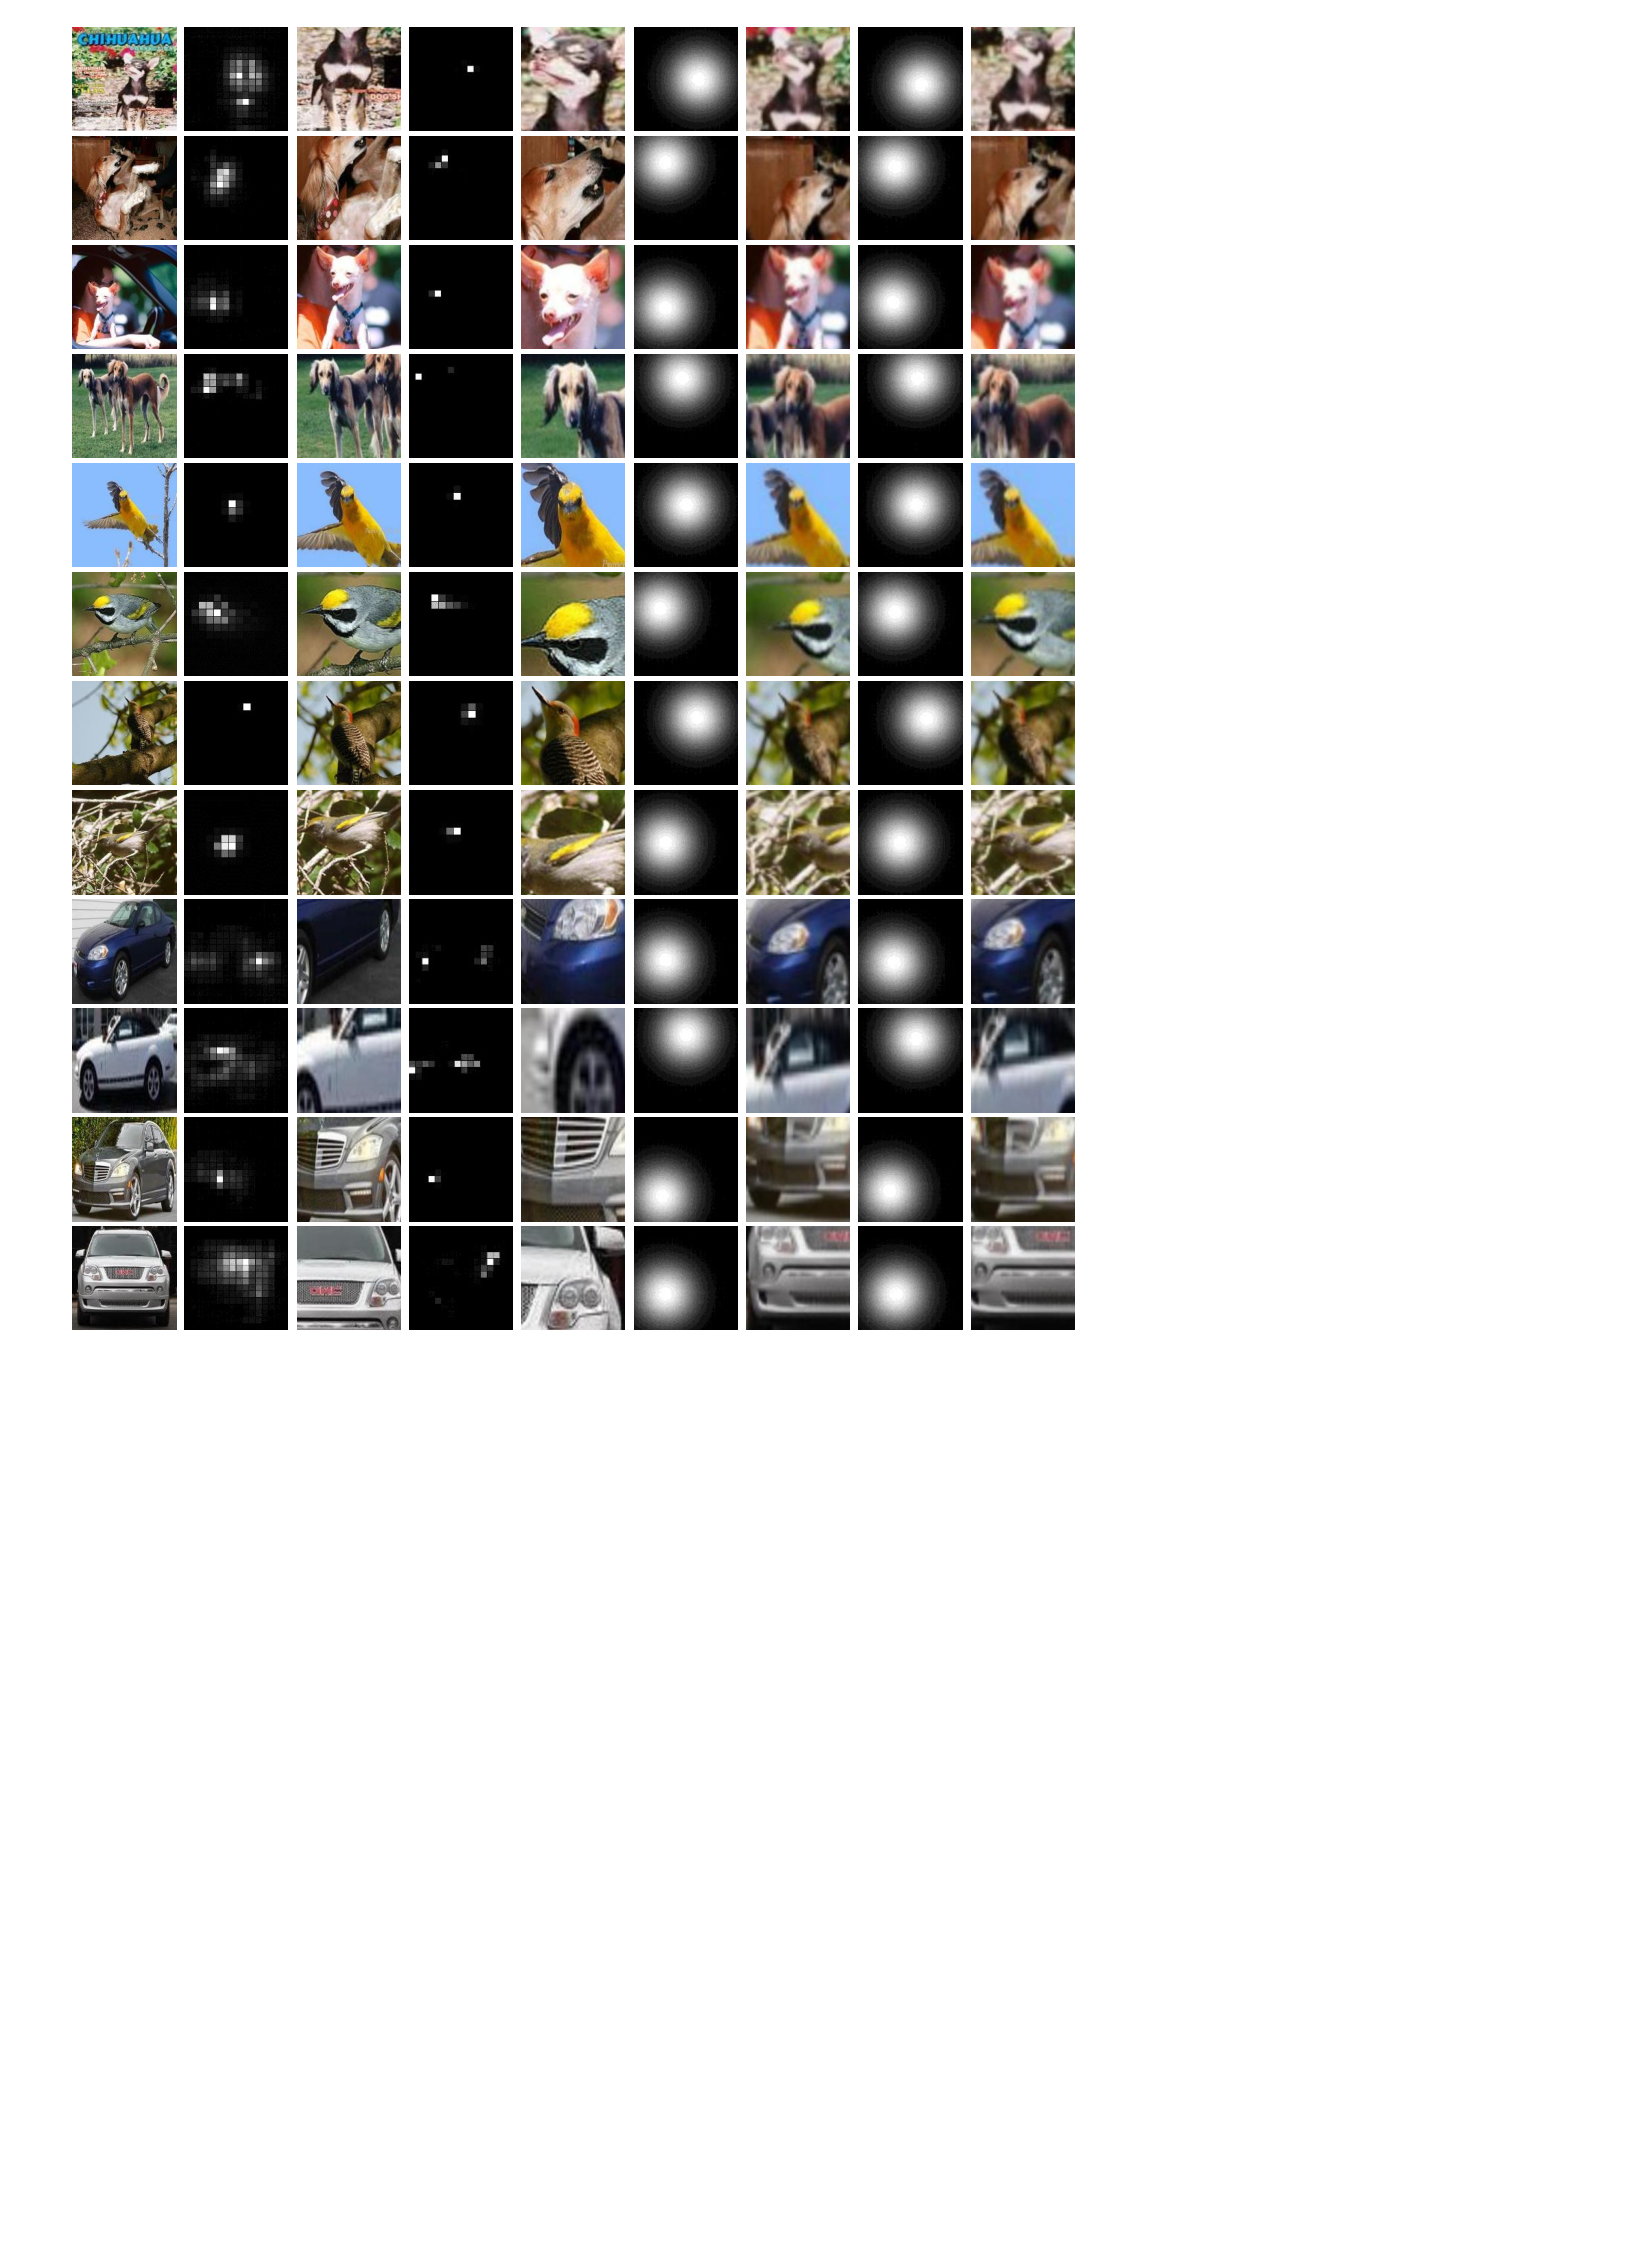
\includegraphics[scale = 0.8]{3.pdf}
\end{center}
\caption{Examples of selected attention regions for the proposed model and  \cite{bd3}.
The first column shows the original image, and the second column and the fourth columns show the outputs of attention localization networks, which are corresponding to $4\times4$ and $8\times8$ attention regions respectively (a lighter region indicates higher score).
The third and the fifth columns show selected attention regions.
The sixth and the eighth columns indicate the heat maps of predicted attention regions in two steps of recurrent attention model \cite{bd3}, and the seventh and ninth columns illustrate the corresponding glimpses (at middle scale).
}\label{fig:attention_illustration}
\end{figure*}

\section{Conclusion}
In this paper, we present attention localization networks for fine-grained recognition.
To improve the performance and to accelerate the speed, fully-convolutional architecture is used and the continuous actions is replaced with discrete actions.
The model is computational efficient and is easy to implement.
We validate the proposed method on three publicly available datasets and show promising results.

In the future, we will explore using differentiable attention model to further increase the training efficiency.


\bibliographystyle{./IEEEtran}
\bibliography{./IEEEabrv,./IEEEexample}
\end{document}

%%% Local Variables:
%%% mode: latex
%%% TeX-master: t
%%% End:
